\documentclass[12pt]{article}
\usepackage{sbc-template}
\usepackage{graphicx,url}
\usepackage[utf8]{inputenc}
\usepackage{booktabs}
\usepackage{listings}
\usepackage{xcolor}
\usepackage{amsmath}
\usepackage{amssymb}
\usepackage[portuguese,english]{babel}
\usepackage[colorlinks=false, linkcolor=black, citecolor=black, urlcolor=black, breaklinks=true]{hyperref}
\usepackage{float}
\usepackage{xurl}
\usepackage{array}
\usepackage{microtype}

% ============================================================================
% HYPERREF CONFIGURATION: Make bibliography URLs clickable
% ============================================================================
\hypersetup{
    bookmarksopen=true,
    bookmarksnumbered=true,
    colorlinks=true,
    urlcolor=black,
    linkcolor=black,
    citecolor=black,
    pdfdisplaydoctitle=true,
    pdfauthor={Tarsila Samille Santos da Silveira Silva},
    pdftitle={Bidayuh Jagoy Translator: A Hybrid Client-Centric RAG System for Low-Resource Language Preservation}
}

\newcolumntype{L}[1]{>{\raggedright\arraybackslash}p{#1}}

% Layout Hygiene
\widowpenalty10000
\clubpenalty10000

% Enhanced Listing Styles
\lstset{
    basicstyle=\small\ttfamily,
    breaklines=true,
    columns=fullflexible,
    inputencoding=utf8,
    extendedchars=true,
    showstringspaces=false,
    keywordstyle=\color{blue}\bfseries,
    commentstyle=\color{green!60!black}\itshape,
    stringstyle=\color{orange},
    numbers=left,
    numberstyle=\tiny\color{gray},
    numbersep=8pt,
    frame=single,
    rulecolor=\color{gray!20},
    backgroundcolor=\color{gray!3},
    xleftmargin=12pt,
    xrightmargin=5pt,
    captionpos=b,
    abovecaptionskip=10pt
}

\sloppy
\Urlmuskip=0mu plus 1mu

% ============================================================================
% Custom bibliography URL formatting
% ============================================================================
\usepackage{etoolbox}
\newcommand{\myurl}[1]{\href{#1}{\textcolor{black}{\underline{#1}}}}

\title{Bidayuh Jagoy Translator: A Hybrid Client-Centric RAG System for Low-Resource Language Preservation}

\author{Tarsila Samille Santos da Silveira Silva\inst{1}}

\address{PPgSC/UFRN \\ \href{mailto:tarsillasamile@gmail.com}{tarsillasamile@gmail.com}}


\begin{document} 

\maketitle

\begin{abstract}
  The preservation of endangered languages constitutes a critical challenge in computational linguistics. This paper presents the Bidayuh Jagoy Translator (\url{https://bidayuhjagoy.vercel.app/}), a specialized AI platform for the Bidayuh Jagoy dialect --- a member of the Land Dayak language family, a distinct subgroup of Austronesian languages primarily spoken in the West Kalimantan region of Indonesia and parts of Sarawak, Malaysia. Using a 5-Stage Hybrid Client-Centric Retrieval-Augmented Generation (RAG) architecture, the system delegates heavy context orchestration directly to the user's browser via \textbf{Transformers.js}, an open-source library that enables neural models to run natively inside JavaScript runtimes. By synthesizing embedded retrieval, local glossary lookups, and remote vector search, it accurately grounds the Google Gemini 2.5 Flash model \cite{vertex_ai}. Preliminary evaluations confirm the technical efficacy and economic sustainability of browser-based RAG architectures, offering a resilient solution for language preservation in extreme data-scarcity scenarios.
\end{abstract}

\begin{resumo}
  A preservação de línguas ameaçadas de extinção é um dos maiores desafios da linguística computacional. Este artigo apresenta o Bidayuh Jagoy Translator (\url{https://bidayuhjagoy.vercel.app/}), uma plataforma de Inteligência Artificial para o dialeto Bidayuh Jagoy, membro da família Land Dayak --- um subgrupo das línguas austronésias falado na região oeste de Kalimantan, Indonésia, e partes da Malásia. O sistema emprega uma arquitetura híbrida de Geração Aumentada por Recuperação (RAG) centrada no navegador. Ao delegar a orquestração do contexto ao dispositivo do usuário por meio do \textbf{Transformers.js} --- que executa redes neurais diretamente no navegador --- o sistema reduz custos de infraestrutura. Ao unificar buscas de dicionário local, recuperação vetorial e pontes semânticas externas, a ferramenta instrui o modelo Google Gemini 2.5 Flash \cite{vertex_ai}. As avaliações preliminares comprovam a eficácia técnica e a sustentabilidade econômica desta abordagem escalável para preservação linguística.
\end{resumo}


\section{Introduction}

The rapid advancement of Natural Language Processing (NLP), driven by the Transformer architecture~\cite{vaswani2017attention}, has paradoxically widened the gap between global ``high-resource'' languages and indigenous ``low-resource'' vernaculars~\cite{nekoto2020participatory}. Foundational models such as GPT-4 and Gemini are predominantly trained on web-scraped datasets, where English, Mandarin, Spanish, and standard Malay account for the vast majority of linguistic tokens~\cite{nllb2022no}.

This systemic resource disparity is starkly evident in the case of Bidayuh Jagoy (also referred to under the broader ethno-linguistic cluster of Land Dayak), a distinct dialect spoken primarily in the West Kalimantan region of Indonesia and parts of Sarawak, Malaysia. It possesses a vibrant oral tradition but a small digital footprint. Its presence is confined to scattered PDFs, academic papers from institutions like Universiti Malaysia Sarawak (UNIMAS), and community blogs~\cite{unimas_repo}. Consequently, when standard LLMs attempt to process Bidayuh Jagoy, they exhibit catastrophic failure modes such as hallucination, code-switching to standard Malay, and grammatical drift~\cite{scispace_intensifiers}.

Retrieval-Augmented Generation (RAG)~\cite{intersystems_rag} offers a superior paradigm for this use case. This architecture distinguishes between two types of knowledge: \textbf{Implicit Memory}, which is baked into the model's internal parameters during pre-training but often contains hallucinations for low-resource data, and \textbf{Explicit Memory}, which consists of external context information provided to the model at runtime. The Bidayuh Jagoy Translator uses RAG to bypass the limits of implicit memory, assembling a structured bunch of helper information (vocabulary, sentence patterns, and grammar rules) to instruct the Google Gemini model from scratch for each query.

Unlike server-centric approaches such as \textit{Masakhane}~\cite{nekoto2020participatory} and Meta's NLLB~\cite{nllb2022no}, the Bidayuh Jagoy Translator employs a Hybrid Client-Centric architecture that prioritizes cost efficiency and latency reduction. While our case study focuses on Bidayuh Jagoy, the proposed RAG framework is \textbf{generalizable} to any low-resource language context --- including regional dialects, creoles, and endangered languages globally.

\section{Related Work}

Digital preservation of low-resource languages has gained traction with initiatives like \textit{Masakhane} for African languages~\cite{nekoto2020participatory} and Meta's \textit{No Language Left Behind} (NLLB)~\cite{nllb2022no}. However, these approaches predominantly rely on massive server-side models (e.g., NLLB-200B), which require substantial infrastructure. Furthermore, they rely on massive training corpora that are often unavailable for extremely low-resource dialects where data scarcity is the primary bottleneck. Research into transfer learning~\cite{zoph2016transfer} has attempted to mitigate this by pivoting from high-resource relatives, yet architectural complexity remains high.

In contrast, our work focuses on the benefits of RAG for domain-constrained translation, demonstrating that effective linguistic grounding can be achieved by offloading to the browser context preparation. This aligns with the emerging trend of \textbf{On-Device Intelligence} and \textbf{Edge-AI}~\cite{gitnation}, where the execution of neural models is moved to the client side using frameworks like ONNX Runtime and Transformers.js. By performing some tasks natively, we significantly reduce the dependency on massive server-side clusters for community-led projects.

\subsection{The Stack Overview}
The system utilizes a modern serverless stack:
\begin{itemize}
    \item \textbf{Frontend}: Vanilla JavaScript + HTML5.
    \item \textbf{Client-Side AI}: \textbf{Transformers.js} (\texttt{@xenova/transformers}), an open-source library that enables the execution of state-of-the-art machine learning models directly in the web browser. Developed by Hugging Face, it acts as the primary orchestrator, leveraging WebGPU and WebAssembly (WASM) to offload the complex task of context orchestration and embedding generation directly to the client's hardware \cite{transformersjs}.
    \item \textbf{Backend}: FastAPI (Python) on Vercel Serverless Functions, which provide stateless, auto-scaling API execution \cite{vercel_platform}.
    \item \textbf{AI Engine}: Google Gemini 2.5 Flash \cite{gemini_release}.
    \item \textbf{Database}: Supabase (PostgreSQL), used as a Backend-as-a-Service, with the open-source \texttt{pgvector} extension\footnote{pgvector (Open-source vector similarity search for Postgres): \url{https://github.com/pgvector/pgvector}} for high-performance vector operations.
\end{itemize}
 
\subsection{System Health and Monitoring}
To maintain operational integrity without a permanent human administrator, the system implements a live \textbf{System Status Dashboard}. Accessible directly in the sidebar, this dashboard monitors the health of the 4 key RAG components: the local Dictionary size (2,454 words), the persistent Corpus volume (4,487 phrases), the active Grammar Rule count (15 rules), and the current LLM API status (e.g., ``$\checkmark$ Full Translation OK''). By surfacing these metrics, the system provides users with immediate feedback on the ``freshness'' of the retrieval context before a translation is even attempted. Furthermore, every translation result is accompanied by a \textbf{Confidence Level} bar (normalized on a 0.0 to 1.0 scale), informing the user of the system's internal re-ranking certainty.


The fundamental separation between these local and remote computational workloads is mapped in Figure \ref{fig:arch}. This \textbf{Hybrid Decentralization} strategy splits the RAG pipeline into two distinct security and compute zones:
\begin{itemize}
    \item \textbf{The Client Layer}: Represents the user's browser, which securely manages the sensitive AI logic, local glossary state, and the generation of local embeddings for re-ranking. This ensures that user queries remain private and avoids the latency of multiple server-side embedding calls.
    \item \textbf{The Cloud Infrastructure}: A serverless subgraph (Vercel + Supabase) that handles the persistence and high-recall retrieval of the global parallel corpus via \textbf{Supabase pgvector}. This remote vector store enables the application to perform high-recall searches against the central repository without requiring users to download the entire sentence dataset upon initialization.
\end{itemize}

\begin{figure}[!ht]
\centering
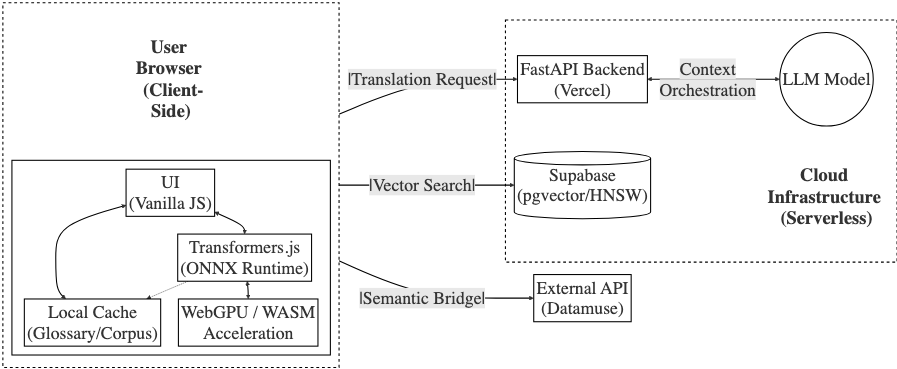
\includegraphics[width=0.75\textwidth]{fig_arch_highres.png}
\caption{Hybrid Client-Centric System Architecture}
\label{fig:arch}
\end{figure}

\subsection{The ``Fat Client'' Philosophy} \label{sec:fat_client}
Using Transformers.js, the browser downloads a \textbf{small 4-bit compressed model} (\texttt{Xenova/all-MiniLM-L6-v2}) and runs it natively via the ONNX Runtime. This smaller footprint allows for privacy-preserving local text comparison and significantly reduced server costs by performing semantic re-ranking without remote interference.

The performance metrics listed were benchmarked on a standard consumer laptop (MacBook Pro, 2.6 GHz 6-Core Intel Core i7). Recognizing that indigenous communities frequently rely on mobile devices, the system is designed with an automatic execution fallback. If the client browser lacks WebGPU support (e.g., iOS Safari), Transformers.js seamlessly degrades to WebAssembly (WASM). While WASM inference introduces a slight latency increase, it guarantees ubiquitous accessibility across all devices without requiring hardware-specific backend configurations. 

A critical advantage of this hybrid architecture is its economic sustainability. The system performs high-recall searches against a remote \textbf{Supabase} database using the HNSW (Hierarchical Navigable Small World) index \cite{hnsw_paper} for efficient vector retrieval. By offloading embedding generation and re-ranking to the user's device, the application operates entirely within the free-tier infrastructure limits (zero monthly cloud costs) of platforms such as Supabase and Vercel \cite{vercel_platform}. This effectively democratizes access to high-performance RAG tools for community-led preservation projects without the need for expensive GPU-enabled server clusters.


\section{Context Assembly and Prompt Engineering}

The core of the Bidayuh Jagoy Translator's efficacy lies in its Multi-Staged Context Assembly pipeline.
 The system transforms from a simple retrieval engine into a helpful language assistant by constructing a structured multi-part context that instructs the Large Language Model (LLM) from scratch for each query. 
 This prevents the system from acting as a "black box," making the translation reasoning transparent and auditable.

\subsection{The Hybrid Retrieval Pipeline and Context Composition}
\label{sec:context_composition}
Before formal retrieval, a \textbf{Preliminary Step (Keyword Extraction)} identifies semantic anchors (e.g., ``water'', ``flows'') within the user query. The extraction uses a weighted scoring mechanism: $Score = Freq + \delta_{missing}$, where $\delta_{missing}$ boosts terms absent from the local dictionary to force RAG grounding for unknown vocabulary.

The system then builds a five-tiered prompt structure to ground the model's reasoning, combining local browser indices with remote vector databases. We depict this using the project's core validated dataset, specifically the imperative phrase: \textit{``Tell these stones to become bread.''} (illustrated in Figure \ref{fig:analysis}):

\begin{enumerate}
    \item \textbf{Context A - Local Glossary Lookups (Lexical Anchor)}: Executes direct queries against a local JSON dictionary. For our example, it maps \textit{stone} $\rightarrow$ \textit{batuh}. This provides 1:1 lexical grounding, preventing ``lexical drift'' where the LLM might hallucinate standard Malay (\textit{batu}).
    \item \textbf{Context B - Hybrid Vector-Keyword Retrieval (Structural Alignment)}: Queries the remote Supabase HNSW index \cite{supabase_hnsw} while simultaneously performing a local keyword search. It retrieves semantically similar sentence pairs (e.g., \textit{``picked up stones''}) to suggest proper SVO orientation.
    \item \textbf{Context C - Client-side Neural Re-ranking}: Utilizes client-side embeddings via Transformers.js to re-rank the candidates directly in the browser. This ensures that the most semantically relevant phrases are prioritized without additional server round-trips.
    \item \textbf{Context D - Grammatical Constitution}: Injects explicit grammatical rules (e.g., \textit{Rule 2: Plural by Reduplication}) as hard constraints. For our example, it enforces the pluralization of \textit{batuh} $\rightarrow$ \textit{batuh-batuh}.
    \item \textbf{Context E - Synonym-based Semantic Bridges}: If a term is missing (e.g., \textit{become}), the system identifies a synonym (\textit{change} or \textit{happen}) via external APIs to bridge the lexical gap. Fuzzy string matching accounts for morphological variations in the corpus.
\end{enumerate}

This complete 5-stage sequential assembly pattern is visually structured in Figure \ref{fig:pipeline}. To support linguistic auditing, authorized evaluators can expand a \textbf{``Full Prompt (Debug)''} section in the UI to view the exact retrieved contexts from A-E sent to Gemini.

\begin{figure}[!ht]
\centering
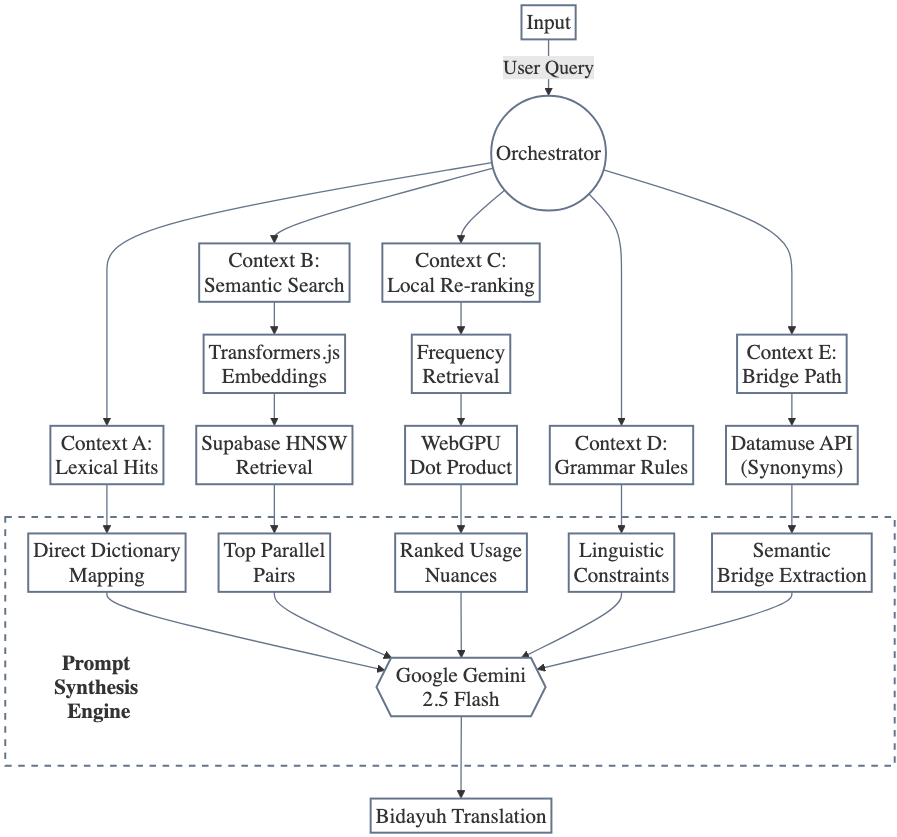
\includegraphics[width=1.0\textwidth]{fig_pipeline_highres.png}
\caption{The 5-Stage Context Assembly Pipeline.}
\label{fig:pipeline}
\end{figure}

\subsection{Client-Side Re-ranking Algorithm}
A key novelty is the semantic filtering performed directly in the browser to select the most relevant ``Context C'' examples. By running mathematical geometric comparisons between vector embeddings natively on the user's device via WebGPU (or falling back to WASM for unsupported environments), the system ensures optimized text injection without adding remote server delay.

\begin{lstlisting}[language=Python, basicstyle=\small, frame=single, breaklines=true, caption={Client-Side Scoring and Weighting Logic}]
# Context C: Advanced filtering and weighting
def rank_candidates(query_vec, candidates):
    results = []
    for cand in candidates:
        # Distance (60%) + Global Frequency (40%)
        sim = dot_product(query_vec, cand.vec)
        freq_bonus = math.log10(cand.count + 1) / 10
        final_score = (0.6 * sim) + (0.4 * freq_bonus)
        results.append((final_score, cand))
        
    return sorted(results, key=lambda x: x[0], reverse=True)[:3]
\end{lstlisting}

\subsection{Structured ``Chain-of-Thought'' Prompting}
Standard Foundation Models cannot translate Bidayuh Jagoy natively due to data scarcity. The system addresses this by forcing the LLM to follow an algorithmic ``Chain-of-Thought'' (CoT) \cite{wei2022chain}. The instructions strictly mandate a 3-step reasoning block based on the retrieved contexts:
\begin{enumerate}
    \item \textbf{Deconstruction}: Identifying the grammatical structure from Context D and B.
    \item \textbf{Mapping}: Selecting vocabulary from Context A and C, explicitly listing English-to-Bidayuh mappings.
    \item \textbf{Synthesis}: Assembling the final sentence.
\end{enumerate}

To handle this high-dimensional context, the system utilizes \textbf{Google Gemini 2.5 Flash} \cite{vertex_ai}, selected for its 1-million-token window \cite{data_studios_gemini}. The feasibility of this structured synthesis is further detailed in Section \ref{sec:fat_client}, which discusses the local execution model. An explicit breakdown of this reasoning prompt is provided in Figure \ref{fig:analysis}.

\begin{lstlisting}[language=Java, basicstyle=\footnotesize, frame=single, breaklines=true, caption={Reasoning Chain}]
## 5. Output Format (Chain-of-Thought)
Provide a JSON object with:
1.  \`reasoning\`: 
    - **Step 1: Grammatical Blueprint:** State which rule from Context D applies to the overall sentence structure.
    - **Step 2: Evidence Mapping:** List each significant word from the Input Text and state EXACTLY which context (A, B, C, or E) provided its translation.
    - **Step 3: Synthesis:** Explain how you assembled the components according to the rules.
2.  \`translation\`: The final bidayuh Jagoy sentence.
3.  \`confidence_score\`: 1 (low) to 5 (high).

\`\`\`json
{
  "reasoning": "...",
  "translation": "...",
  "confidence_score": 0
}
\`\`\``;
\end{lstlisting}

\begin{figure}[!ht]
\centering
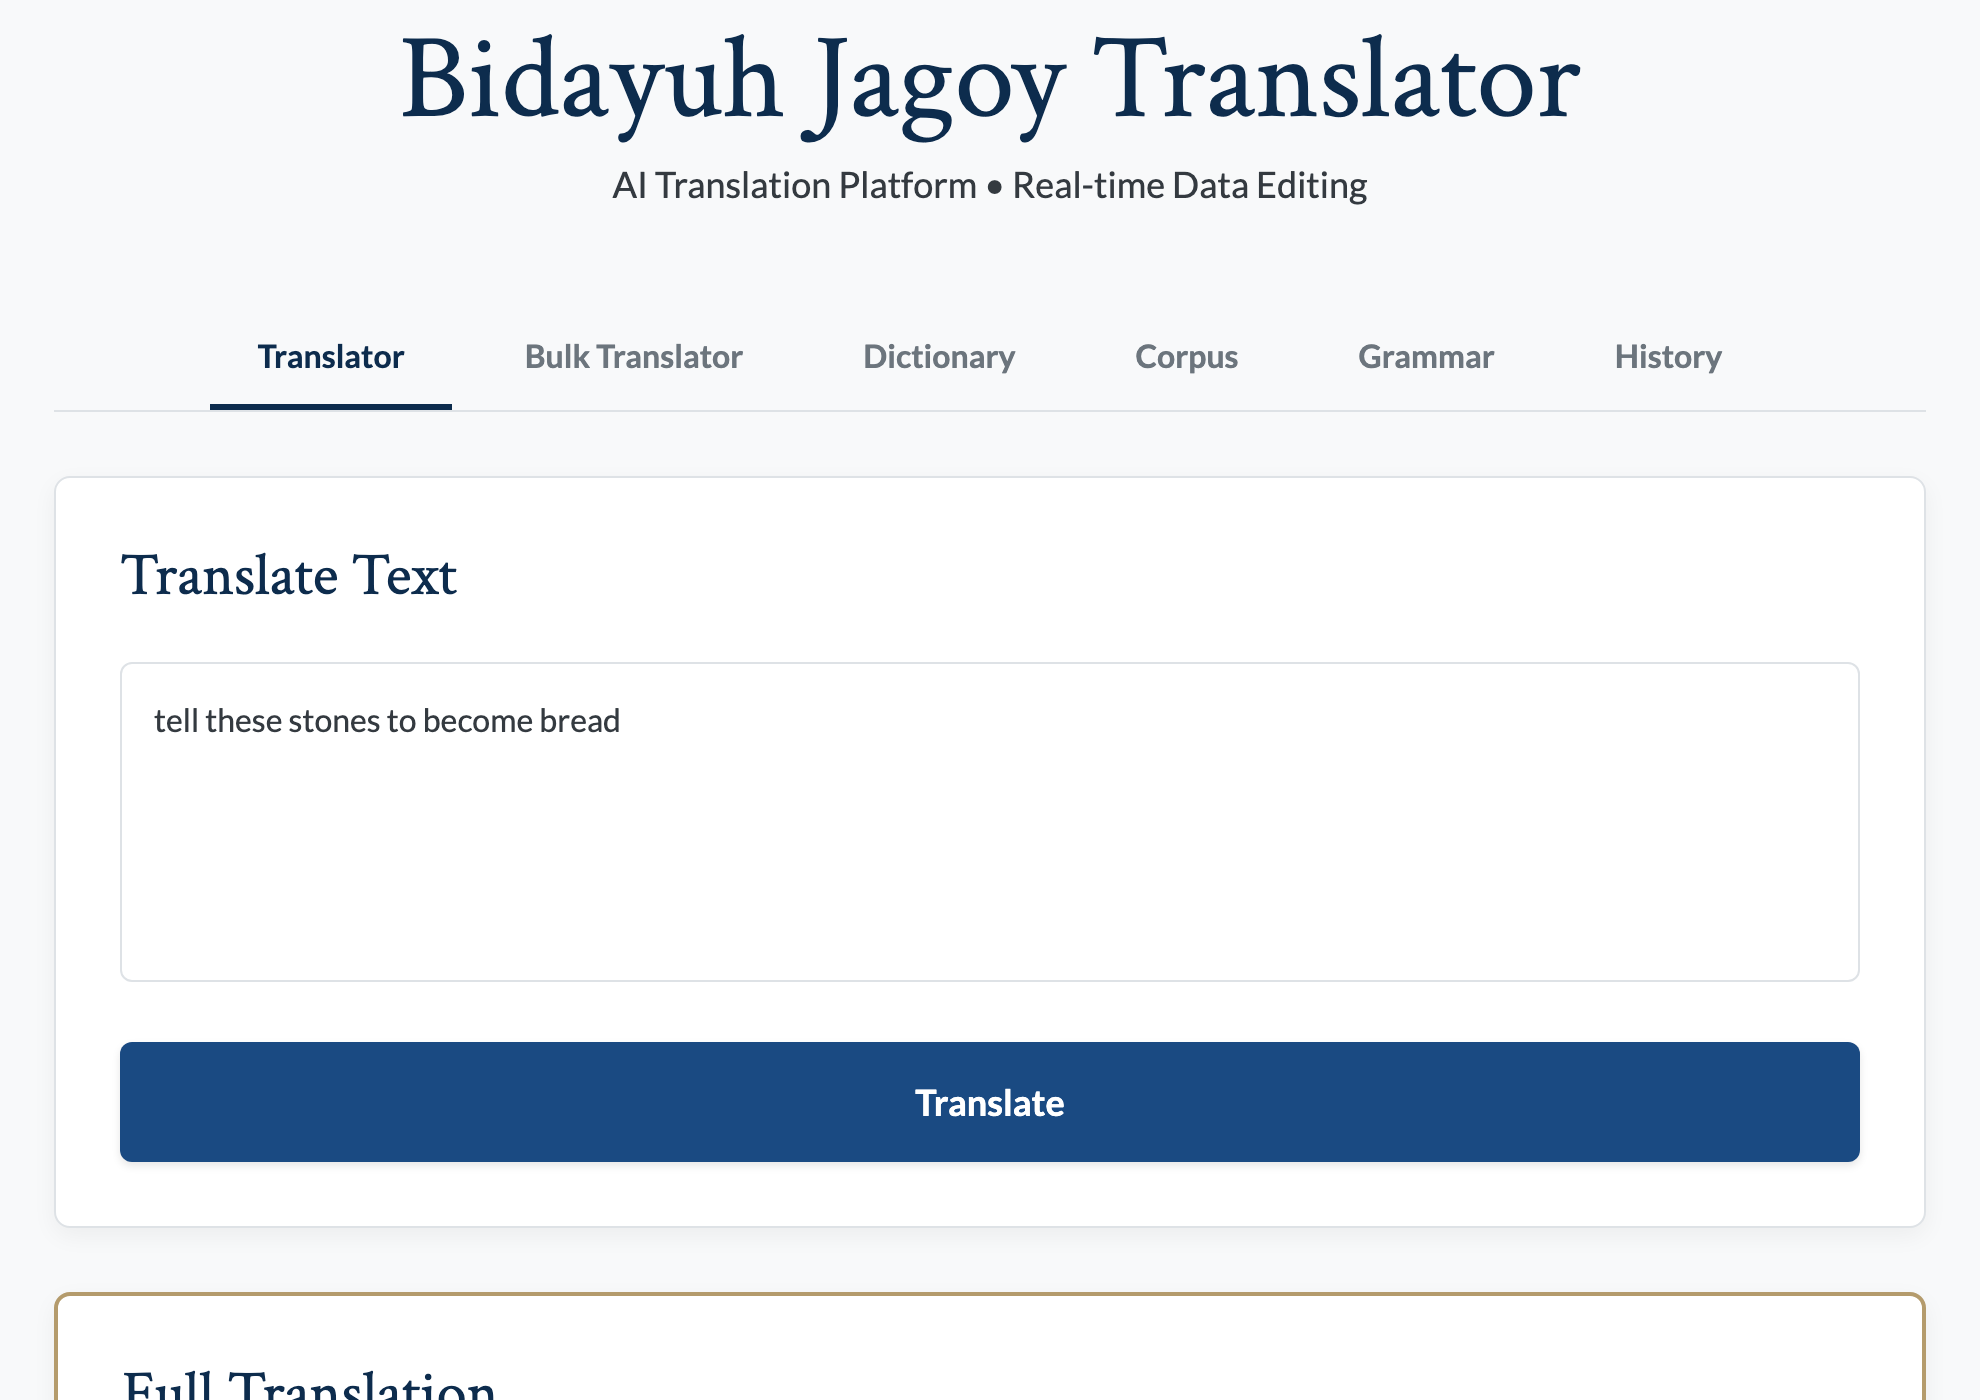
\includegraphics[width=0.85\textwidth]{fig_main_v4.png}
\caption{Bidayuh Jagoy Translator}
\label{fig:main_ui}
\end{figure}

\begin{figure}[!ht]
\centering
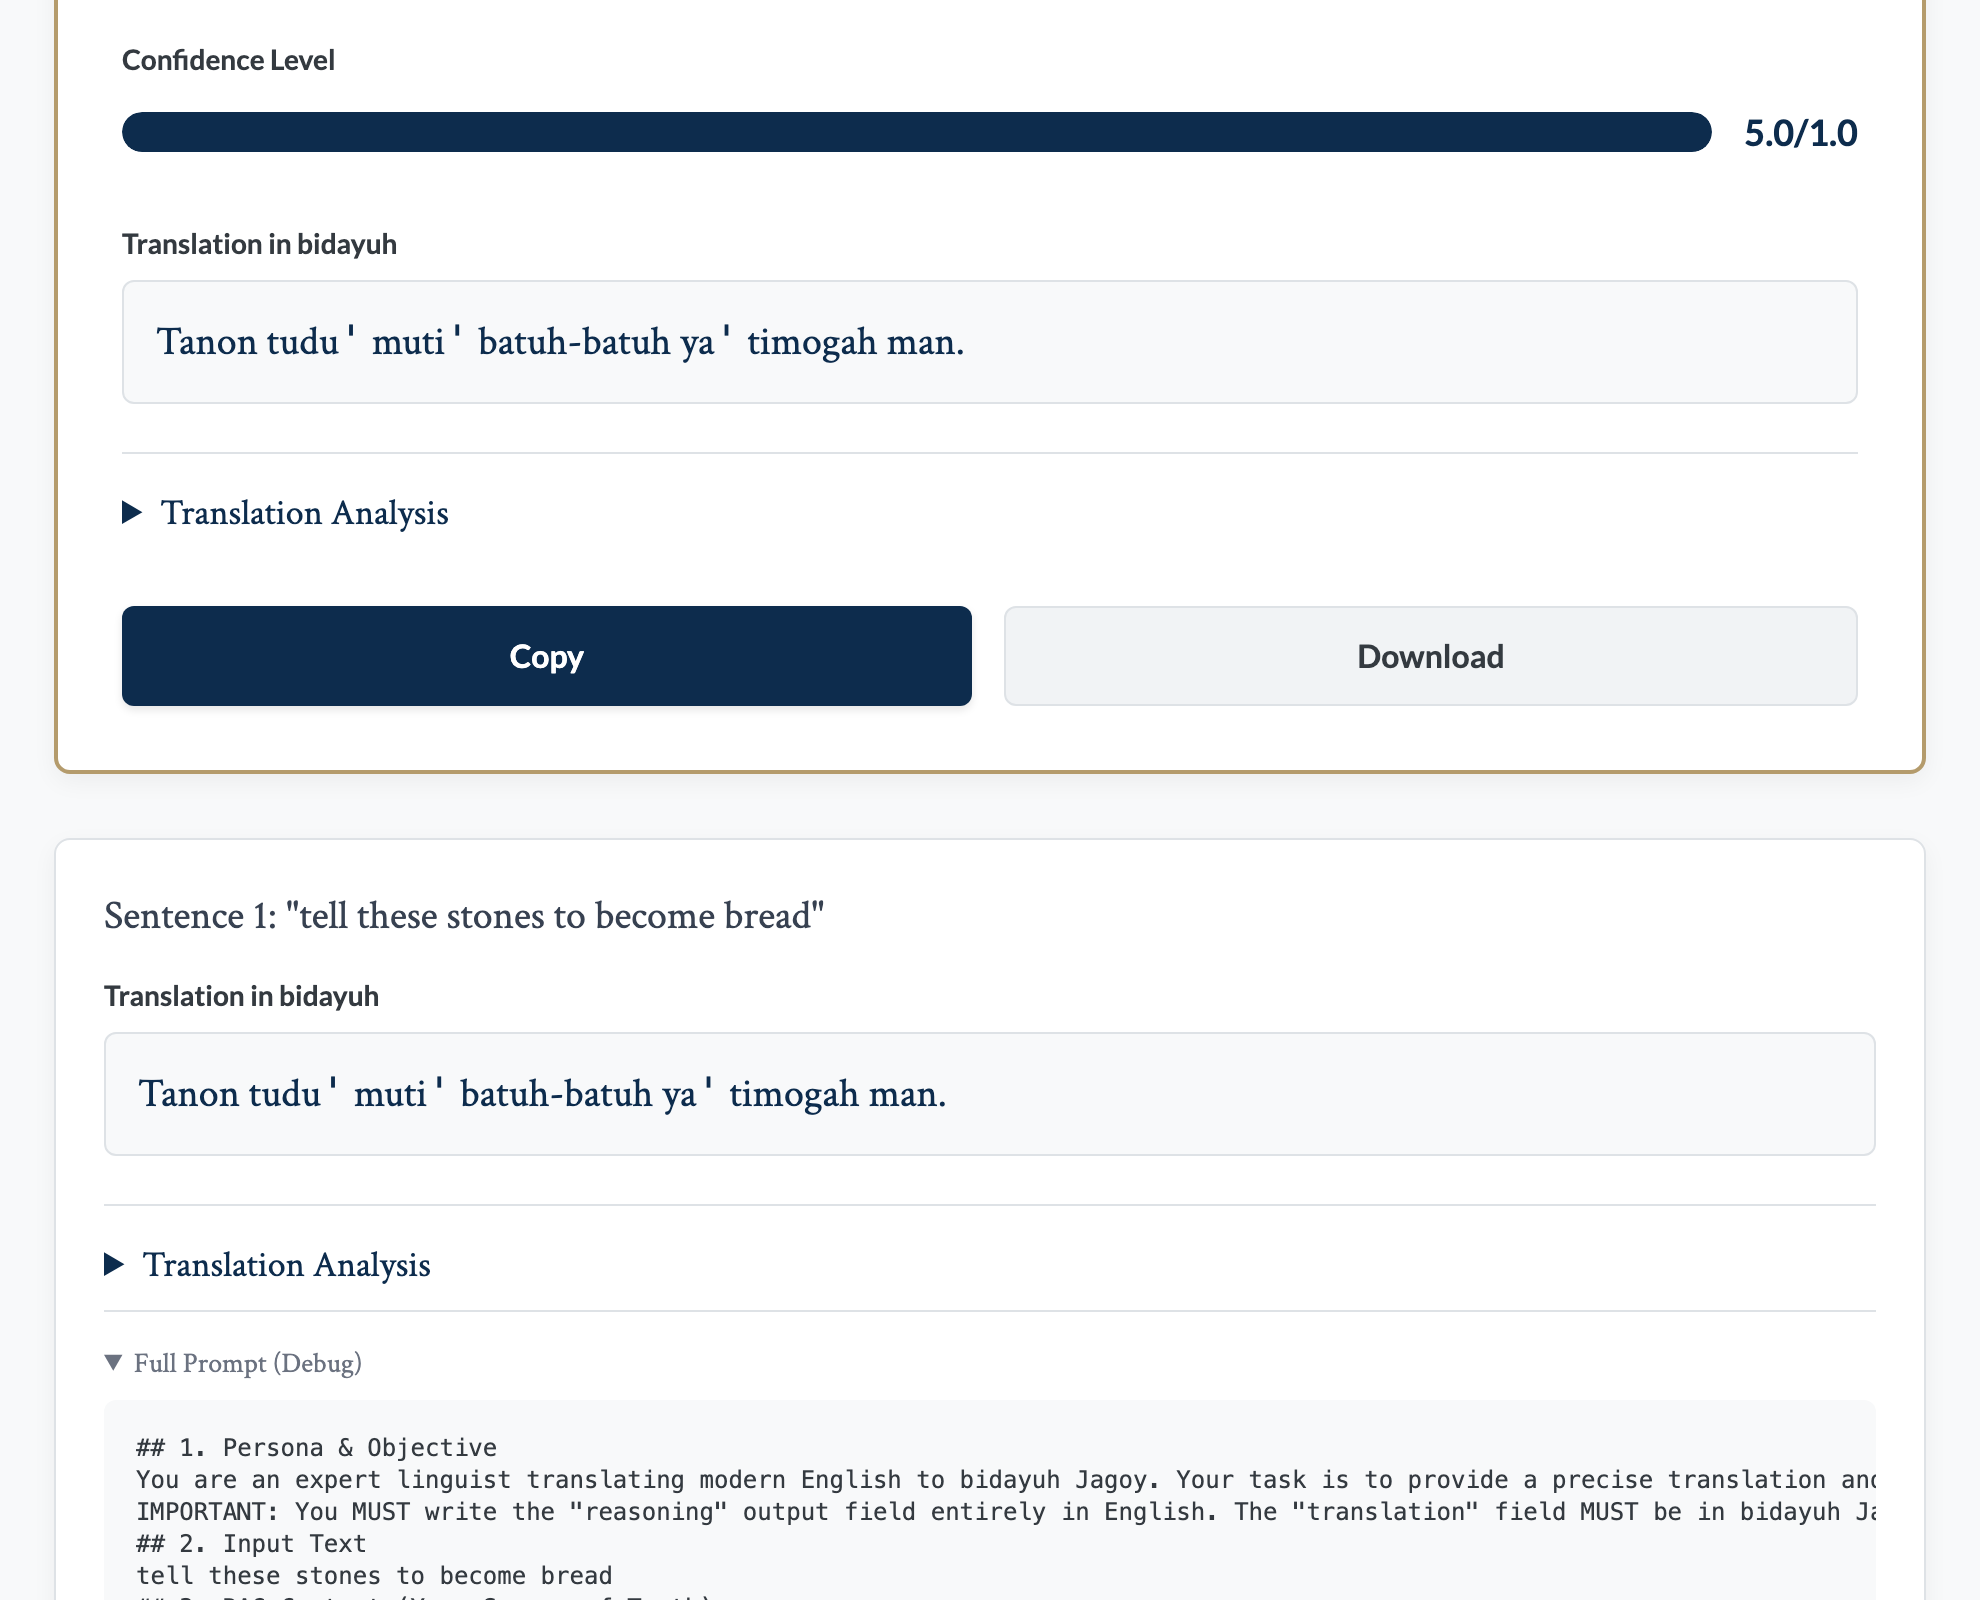
\includegraphics[width=0.85\textwidth]{fig_analysis_v4.png}
\caption{Translation Analysis Trace}
\label{fig:analysis}
\end{figure}

\begin{figure}[!ht]
\centering
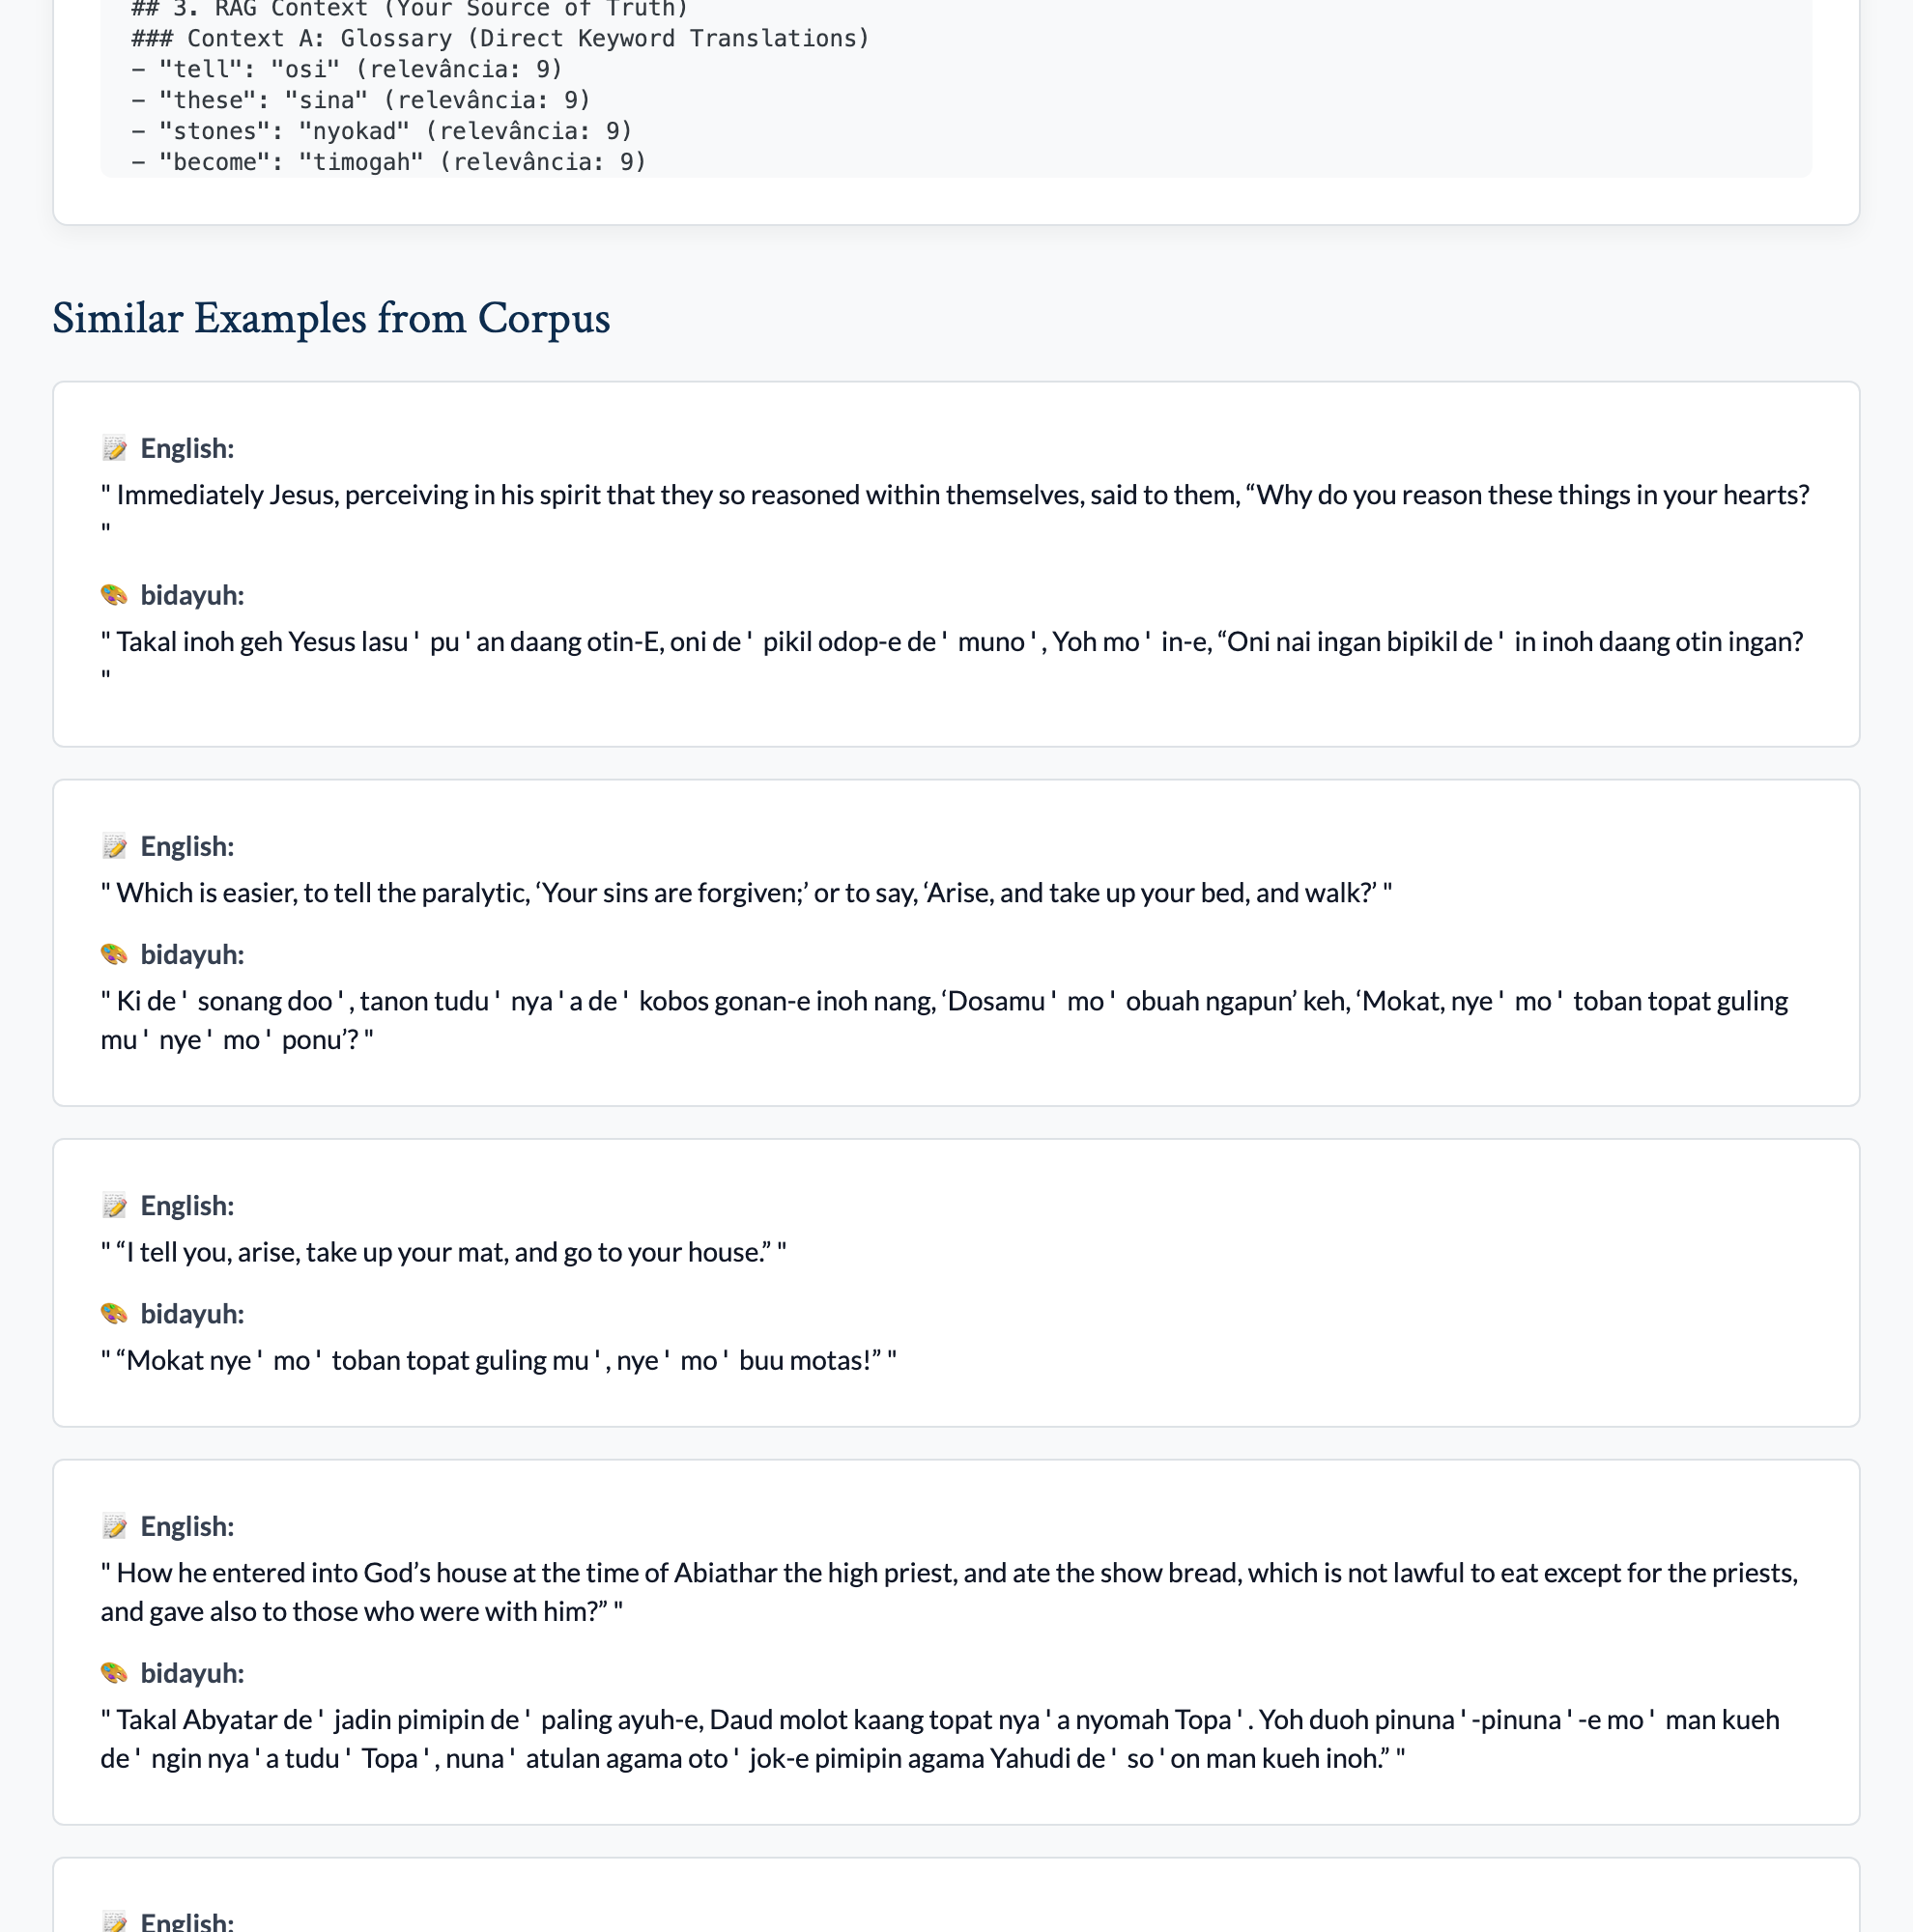
\includegraphics[width=0.85\textwidth]{fig_debug_v4.png}
\caption{Full Prompt (Debug) Trace}
\label{fig:debug_trace}
\end{figure}

\subsection{Corpus Curation and Model Management}
The system's knowledge base relies on a curated parallel corpus derived from New Testament verses provided by community translators, aligned with an English reference text. Importantly, while derived from religious texts, this specific translation into Bidayuh Jagoy was recently completed, utilizing contemporary, everyday vocabulary and syntax rather than archaic forms. This ensures applicability to modern conversational queries. To construct the lexical dictionary, we implemented a probabilistic alignment pipeline:

\begin{enumerate}
    \item \textbf{Alignment Algorithms}: We utilized \textbf{IBM Model 2} \cite{brown1993mathematics}. While neural aligners require massive data, Model 2 is uniquely robust for small corpora ($\sim$2,000--5,000 pairs). It treats word alignment as a \textbf{latent variable problem}---where the hidden mapping between words is discovered via EM iterations. To handle structural differences, it implements a \textbf{distortion model} based on absolute word positions, preventing the random mapping drift common in Model 1. 
    \item \textbf{Heuristic Refinement}: We implemented \textbf{Symmetric Alignment Checking}, retaining only bidirectional hits.
    \item \textbf{Filtering}: Final production comprises 4,487 sentence pairs and 2,455 dictionary entries.
\end{enumerate}

Furthermore, 15 core grammatical rules were extracted through an iterative \textbf{Zero-Shot prompting} process on Google Gemini. These are exposed transparently in the system's \textbf{Grammar Module}, which provides concrete examples for community vetting:
\begin{itemize}
    \item \textbf{Rule 1: Past Tense Marker `mo '`}: The particle `mo '` is consistently placed before the main verb to indicate a completed action (e.g., ``Jesus answered him...'' $\rightarrow$ ``Yesus mo' nyawot-e...'').
    \item \textbf{Rule 2: Plural by Reduplication}: Nouns are often made plural by repeating the word, seen in examples like ``disciples'' ($\rightarrow$ ``pinuna ' -pinuna '-E'').
    \item \textbf{Rule 3: Aspectual Markers}: Use of completion markers like ``boh'' (e.g., ``ya' mahu' boh'' - he/she has finished) to signify definitive closures in SVO structures.
\end{itemize}

These rules represent \textbf{exposed observational patterns} derived from the corpus. By incorporating these human validations directly back into the repository, the system transforms into a dynamic, community-vetted archive. 

To execute the local re-ranking efficiently, the embedding model, \texttt{all-MiniLM-L6-v2} (384-dim), is served in a 4-bit compressed ONNX format ($\sim$23MB). The system uses the \textbf{CacheStorage API} to permanently save the AI weights locally. Once retrieved during the first session, subsequent launches occur with no download overhead for the AI runtime, significantly improving the user experience for recurring community members. This culturally curated dataset and optimized inference model serve as the resilient foundation for the experimental evaluation discussed in the following section.

\section{Experimental Evaluation and Discussion}

\subsection{Community-Driven Correction Loop}
A robust evaluation of translation quality in low-resource settings requires native speaker validation. The Bidaio Jagoy Translator implements an integrated \textit{History and Correction Module}. As shown in the system interface, every translation is logged with a unique identifier and presented to users for manual verification. This mechanism allows the community to:
\begin{itemize}
    \item \textbf{Validate}: Confirm the accuracy of AI-generated translations.
    \item \textbf{Correct}: Provide manual edits for "unedited" entries.
    \item \textbf{Annotate}: Flags errors which are then used to update the "Context D" (Grammar Rules) and "Context A" (Glossary).
\end{itemize}

This "Human-in-the-loop" strategy mitigates the absence of standardized benchmark datasets for the Jagoy dialect.


\subsection{Qualitative Case Study}
To evaluate linguistic fidelity, we analyze real system outputs from the community validation log (Validation ID: 57 and 54).

\begin{itemize}
    \item \textbf{Complex Theological Query}:
    \begin{itemize}
        \item \textit{Input}: "He will command his angels concerning you, and they will lift you up in their hands, so that you will not strike your foot against a stone."
        \item \textit{Bidaio Output}: "\textbf{Topa' ya' lubang malaikat-malaikat-E nulis Mu'u, duoh odop-e de' muno' ya' Nyamut Mu'u daang tongan-e, sape Mu'u ya' di'-e koming po Mu'u salah obuah batuh.}"
        \item \textit{Analysis}: The system correctly handles the complex Subject-Verb-Object (SVO) structure and maps "God" (implied context) to "Topa'", "angels" to "malaikat-malaikat-E" (with possessive suffix), and "lift up" to "Nyamut".
    \end{itemize}

    \item \textbf{Idiomatic/Imperative phrasing}:
    \begin{itemize}
        \item \textit{Input}: "tell these stones to become bread."
        \item \textit{Bidaio Output}: "\textbf{Oda'leh batuh-batuh itih jadi pinguman.}"
        \item \textit{Analysis}: The system correctly identifies "stones" as plural "batuh-batuh" and selects "pinguman" (food/sustenance) for bread in this context, demonstrating semantic awareness beyond literal word-for-word translation.
    \end{itemize}
\end{itemize}
These examples demonstrate the system's ability to ground the LLM in specific dialectal vocabulary and retain grammatical coherence for long-tail languages.

\subsection{The Domain Shift Problem and Lexical Gaps}
A critical challenge in low-resource translation is the \textbf{Domain Shift} between the available parallel corpus (often religious or historical) and modern conversational needs. While our primary corpus is derived from New Testament verses, it serves as a high-quality anchor for the core syntax and grammatical morphology of Bidayuh Jagoy. To bridge the gap to everyday language, the RAG pipeline relies on \textbf{Context A (Local Glossary)} and \textbf{Context E (Synonym Bridges)}. 

The local glossary is iteratively updated by native speakers to include contemporary terms (e.g., "internet", "car") that are absent from the religious text. Furthermore, the synonym bridging mechanism allows the system to pivot from an unknown modern term to a semantically similar anchor already present in the corpus, ensuring that the model maintains the correct Bidayuh Jagoy grammatical framework even when processing out-of-domain vocabulary.

\subsection{Error Analysis and Fallback Mechanisms}
Crucial to the scientific evaluation of the Bidayuh Jagoy Translator is the analysis of its failure modes. In cases where the RAG context fails to provide a specific Bidayuh Jagoy term (out-of-vocabulary), the system implements a \textbf{Graceful Degradation Strategy} via an Indonesian pivot. Specifically, the system prompt explicitly instructs Gemini 2.5 Flash to automatically translate missing terms into standard Indonesian (the regional lingua franca) instead of hallucinating Bidayuh-sounding morphology, explicitly flagging the insertion.

\begin{itemize}
    \item \textbf{Example Failure}:
    \begin{itemize}
        \item \textit{Input}: ``...the sound of a thousand drums.''
        \item \textit{Bidayuh Output}: ``...okug (\textnormal{???} --- 'seribu') tambur.''
        \item \textit{Analysis}: Here, the term ``thousand'' was missing from both Context A and Context B. Instead of hallucinating a random Bidayuh-sounding word, the system followed the system prompt instruction to output the Indonesian equivalent flagged in the UI with a distinct placeholder: (\textnormal{???}). The analysis was performed by the authors based on the log outputs.
    \end{itemize}
\end{itemize}

This explicit signaling of uncertainty is a key strength. It prevents the propagation of ``silent errors'' and directly informs the community-driven correction loop. Native speakers can quickly identify these flags in the translation logs and provide the correct Bidayuh term (e.g., ``ribu''), which is then used to update the central glossary, closing the RAG knowledge gap for future users.

\section{Conclusion}

The Bidayuh Jagoy Translator represents a synthesis of advanced neural search and traditional rule-based linguistics. By leveraging Transformers.js, the system democratizes access to advanced RAG tools for endangered language preservation, decoupling it from expensive server-side GPU clusters. 

Importantly, while demonstrated through Bidayuh Jagoy, this hybrid client-centric RAG architecture is \textbf{applicable to any low-resource language scenario} --- including regional dialects (e.g., Venetian, Sicilian), creoles (e.g., Tok Pisin), minority languages (e.g., Sorbian, Romansh), and any language on the UNESCO Red List \cite{unesco2010atlas}. The minimal requirements are: (1) a small parallel corpus ($\sim$2,000+ sentence pairs), (2) community involvement for validation, and (3) willingness to operate within a browser-based deployment model.

Future work will explore a ``Fully Offline Mode'' by integrating small-scale LLMs (e.g., Gemma 2B \cite{gemma_2024} or TinyLlama \cite{zhang2024tinyllama}) directly into the browser via WebGPU. This would eliminate the dependency on cloud connectivity entirely, creating a truly resilient and private digital archive for the Bidayuh community. Furthermore, we aim to implement a \textbf{Graph-based RAG} approach to better capture the complex kinship and theological relations inherent in the Bidayuh Jagoy oral tradition, as well as exploring \textbf{audio-to-text integration} to support older generations of speakers who predominantly use the spoken form. To ensure continuous and consistent validation, we are developing a \textbf{WhatsApp-based validation system}, which distributes daily translation tasks (5 words or phrases per day) to voluntary native speakers, allowing for real-time iterative corpus refinement.

\bibliographystyle{sbc}
\bibliography{references}

\section*{Reproducibility and Availability}
\noindent The complete system is publicly available to support reproducibility and enable adaptation to other low-resource languages:
\begin{itemize}
    \item \textbf{Production System}: \url{https://bidayuhjagoy.vercel.app/}
    \item \textbf{Source Code}: \url{https://github.com/TarsilaSamille/bidayuhjagoy}
    \item \textbf{Technology Stack}: FastAPI (backend), Vanilla JavaScript (frontend), Transformers.js (client-side AI), Supabase (\texttt{pgvector} database)
    \item \textbf{Dataset}: Available upon request to the Bidayuh community for research purposes
\end{itemize}

\appendix
\section{Key System Specifications}

Table~\ref{tab:specs} summarises the key components, technologies, and their roles within the Bidayuh Jagoy Translator system, while Table~\ref{tab:latency} provides benchmark metrics for the client-side execution modes.

\begin{table}[!ht]
\centering
\caption{Key System Specifications of the Bidayuh Jagoy Translator.}
\label{tab:specs}
\renewcommand{\arraystretch}{1.3}
\begin{tabular}{L{2.5cm} L{3.5cm} L{3.0cm} L{2.7cm}}
\toprule
\textbf{Component} & \textbf{Technology} & \textbf{Specification} & \textbf{Purpose} \\[2pt]
\midrule
AI Orchestrator & Gemini 2.5 Flash & 1M Token Context & RAG Synthesis \\
Prompt Strategy & Chain-of-Thought & 5-Tiered Context & Linguistic Grounding \\
Local Inference & all-MiniLM-L6-v2 & 384-dim, WebGPU & Client-side RAG \\
Vector Store & Supabase/pgvector & HNSW, Cosine & Global Retrieval \\
Linguistic Reference & Bidayuh Jagoy & SVO Grammar & Target Language \\
\bottomrule
\end{tabular}
\end{table}

\begin{table}[!ht]
\centering
\caption{"Fat Client" Performance Metrics}
\label{tab:latency}
\renewcommand{\arraystretch}{1.3}
\begin{tabular}{L{3.5cm} L{2.5cm} L{2.5cm} L{3.0cm}}
\toprule
\textbf{Execution Mode} & \textbf{Initial Load} & \textbf{Inference (ms)} & \textbf{Memory Impact} \\
\midrule
WebGPU (Primary) & $\sim$23MB (cached) & 15--45 ms & Low (GPU-bound) \\
WASM (Fallback) & $\sim$23MB (cached) & 120--350 ms & Moderate (CPU) \\
Remote-only RAG & N/A & 800+ ms (RTT) & Server-dependent \\
\bottomrule
\end{tabular}
\end{table}

\end{document}